\documentclass[11pt,preprint]{elsarticle}

\usepackage{lmodern}
%%%% My spacing
\usepackage{setspace}
\setstretch{1.2}
\DeclareMathSizes{12}{14}{10}{10}

% Wrap around which gives all figures included the [H] command, or places it "here". This can be tedious to code in Rmarkdown.
\usepackage{float}
\let\origfigure\figure
\let\endorigfigure\endfigure
\renewenvironment{figure}[1][2] {
    \expandafter\origfigure\expandafter[H]
} {
    \endorigfigure
}

\let\origtable\table
\let\endorigtable\endtable
\renewenvironment{table}[1][2] {
    \expandafter\origtable\expandafter[H]
} {
    \endorigtable
}


\usepackage{ifxetex,ifluatex}
\usepackage{fixltx2e} % provides \textsubscript
\ifnum 0\ifxetex 1\fi\ifluatex 1\fi=0 % if pdftex
  \usepackage[T1]{fontenc}
  \usepackage[utf8]{inputenc}
\else % if luatex or xelatex
  \ifxetex
    \usepackage{mathspec}
    \usepackage{xltxtra,xunicode}
  \else
    \usepackage{fontspec}
  \fi
  \defaultfontfeatures{Mapping=tex-text,Scale=MatchLowercase}
  \newcommand{\euro}{€}
\fi

\usepackage{amssymb, amsmath, amsthm, amsfonts}

\def\bibsection{\section*{References}} %%% Make "References" appear before bibliography


\usepackage[numbers]{natbib}

\usepackage{longtable}
\usepackage[margin=2.3cm,bottom=2cm,top=2.5cm, includefoot]{geometry}
\usepackage{fancyhdr}
\usepackage[bottom, hang, flushmargin]{footmisc}
\usepackage{graphicx}
\numberwithin{equation}{section}
\numberwithin{figure}{section}
\numberwithin{table}{section}
\setlength{\parindent}{0cm}
\setlength{\parskip}{1.3ex plus 0.5ex minus 0.3ex}
\usepackage{textcomp}
\renewcommand{\headrulewidth}{0.2pt}
\renewcommand{\footrulewidth}{0.3pt}

\usepackage{array}
\newcolumntype{x}[1]{>{\centering\arraybackslash\hspace{0pt}}p{#1}}

%%%%  Remove the "preprint submitted to" part. Don't worry about this either, it just looks better without it:
\makeatletter
\def\ps@pprintTitle{%
  \let\@oddhead\@empty
  \let\@evenhead\@empty
  \let\@oddfoot\@empty
  \let\@evenfoot\@oddfoot
}
\makeatother

 \def\tightlist{} % This allows for subbullets!

\usepackage{hyperref}
\hypersetup{breaklinks=true,
            bookmarks=true,
            colorlinks=true,
            citecolor=blue,
            urlcolor=blue,
            linkcolor=blue,
            pdfborder={0 0 0}}


% The following packages allow huxtable to work:
\usepackage{siunitx}
\usepackage{multirow}
\usepackage{hhline}
\usepackage{calc}
\usepackage{tabularx}
\usepackage{booktabs}
\usepackage{caption}


\newenvironment{columns}[1][]{}{}

\newenvironment{column}[1]{\begin{minipage}{#1}\ignorespaces}{%
\end{minipage}
\ifhmode\unskip\fi
\aftergroup\useignorespacesandallpars}

\def\useignorespacesandallpars#1\ignorespaces\fi{%
#1\fi\ignorespacesandallpars}

\makeatletter
\def\ignorespacesandallpars{%
  \@ifnextchar\par
    {\expandafter\ignorespacesandallpars\@gobble}%
    {}%
}
\makeatother


% definitions for citeproc citations
\NewDocumentCommand\citeproctext{}{}
\NewDocumentCommand\citeproc{mm}{%
\href{\#cite.\detokenize{#1}}{#2}\nocite{#1}}

\makeatletter
% allow citations to break across lines
\let\@cite@ofmt\@firstofone
% avoid brackets around text for \cite:
\def\@biblabel#1{}
\def\@cite#1#2{{#1\if@tempswa , #2\fi}}
\makeatother
\newlength{\cslhangindent}
\setlength{\cslhangindent}{1.5em}
\newlength{\csllabelwidth}
\setlength{\csllabelwidth}{3em}
\newenvironment{CSLReferences}[2] % #1 hanging-indent, #2 entry-spacing
{\begin{list}{}{%
	\setlength{\itemindent}{0pt}
	\setlength{\leftmargin}{0pt}
	\setlength{\parsep}{0pt}
	% turn on hanging indent if param 1 is 1
	\ifodd #1
	\setlength{\leftmargin}{\cslhangindent}
	\setlength{\itemindent}{-1\cslhangindent}
	\fi
	% set entry spacing
	\setlength{\itemsep}{#2\baselineskip}}}
{\end{list}}

\usepackage{calc}
\newcommand{\CSLBlock}[1]{\hfill\break\parbox[t]{\linewidth}{\strut\ignorespaces#1\strut}}
\newcommand{\CSLLeftMargin}[1]{\parbox[t]{\csllabelwidth}{\strut#1\strut}}
\newcommand{\CSLRightInline}[1]{\parbox[t]{\linewidth - \csllabelwidth}{\strut#1\strut}}
\newcommand{\CSLIndent}[1]{\hspace{\cslhangindent}#1}


\urlstyle{same}  % don't use monospace font for urls
\setlength{\parindent}{0pt}
\setlength{\parskip}{6pt plus 2pt minus 1pt}
\setlength{\emergencystretch}{3em}  % prevent overfull lines
\setcounter{secnumdepth}{5}

%%% Use protect on footnotes to avoid problems with footnotes in titles
\let\rmarkdownfootnote\footnote%
\def\footnote{\protect\rmarkdownfootnote}
\IfFileExists{upquote.sty}{\usepackage{upquote}}{}

%%% Include extra packages specified by user

%%% Hard setting column skips for reports - this ensures greater consistency and control over the length settings in the document.
%% page layout
%% paragraphs
\setlength{\baselineskip}{12pt plus 0pt minus 0pt}
\setlength{\parskip}{12pt plus 0pt minus 0pt}
\setlength{\parindent}{0pt plus 0pt minus 0pt}
%% floats
\setlength{\floatsep}{12pt plus 0 pt minus 0pt}
\setlength{\textfloatsep}{20pt plus 0pt minus 0pt}
\setlength{\intextsep}{14pt plus 0pt minus 0pt}
\setlength{\dbltextfloatsep}{20pt plus 0pt minus 0pt}
\setlength{\dblfloatsep}{14pt plus 0pt minus 0pt}
%% maths
\setlength{\abovedisplayskip}{12pt plus 0pt minus 0pt}
\setlength{\belowdisplayskip}{12pt plus 0pt minus 0pt}
%% lists
\setlength{\topsep}{10pt plus 0pt minus 0pt}
\setlength{\partopsep}{3pt plus 0pt minus 0pt}
\setlength{\itemsep}{5pt plus 0pt minus 0pt}
\setlength{\labelsep}{8mm plus 0mm minus 0mm}
\setlength{\parsep}{\the\parskip}
\setlength{\listparindent}{\the\parindent}
%% verbatim
\setlength{\fboxsep}{5pt plus 0pt minus 0pt}



\begin{document}



\begin{frontmatter}  %

\title{Macroeconomics Assignment}

% Set to FALSE if wanting to remove title (for submission)




\author[Add1]{Liam Andrew Beattie}
\ead{22562435@sun.ac.za}





\address[Add1]{Macroeconomics 871, Stellenbosch University, South
Africa}


\begin{abstract}
\small{
Abstract to be written here. The abstract should not be too long and
should provide the reader with a good understanding what you are writing
about. Academic papers are not like novels where you keep the reader in
suspense. To be effective in getting others to read your paper, be as
open and concise about your findings here as possible. Ideally, upon
reading your abstract, the reader should feel he / she must read your
paper in entirety.
}
\end{abstract}

\vspace{1cm}





\vspace{0.5cm}

\end{frontmatter}

\setcounter{footnote}{0}



%________________________
% Header and Footers
%%%%%%%%%%%%%%%%%%%%%%%%%%%%%%%%%
\pagestyle{fancy}
\chead{}
\rhead{}
\lfoot{}
\rfoot{\footnotesize Page \thepage}
\lhead{}
%\rfoot{\footnotesize Page \thepage } % "e.g. Page 2"
\cfoot{}

%\setlength\headheight{30pt}
%%%%%%%%%%%%%%%%%%%%%%%%%%%%%%%%%
%________________________

\headsep 35pt % So that header does not go over title




Start writing about what you are planning to do, note that this is an
assignment and what it is (introduction vibes)

Please give credit: I haved used an R package from Mati
(\citeproc{ref-Mati2019}{2019})

\section{Model Specification}\label{model-specification}

\#\# Core RBC Foundations

Above could note be a heading on itself. Just a paragraph that it is a
core rbc foundations and what that means.

Note that capital letters denote nominal amounts and lowercase denote
real values.

\begin{equation}
C_t \;=\; P_t \, c_t,
\qquad
I_t \;=\; P_t \, i_t
\label{nominal_definitions}
\end{equation}

\begin{equation}
\max_{\{C_t,\,h_t,\,M_t,\,B_t,\,K_t,\,I_t\}}
\mathbb{E}_0 \sum_{t=1}^{\infty} \beta^{t-1}
\left[
\frac{\Bigl(\frac{C_t}{P_t} - \eta\,\frac{C_{t-1}}{P_{t-1}}\Bigr)^{1-\theta}}{1-\theta}
\;-\;\chi\,\frac{h_t^{1+\gamma}}{1+\gamma}
\;+\;\psi\,\ln\!\Bigl(\frac{M_t}{P_t}\Bigr)
\right]
\label{lifetime_utility_nominal}
\end{equation}

\begin{equation}
C_t \;+\; I_t \;+\; B_t \;+\; M_t
\;\le\;
R^B_{\,t-1}\,B_{t-1}
\;+\; M_{t-1}
\;+\; W_t\,h_t
\;+\; R^k_t\,K_{t-1}
\;+\; \Pi_t
\;-\; P_t\,\tau_t
\label{flow_constraint_nominal}
\end{equation}

\begin{equation}
K_t
\;=\;
(1 - \delta)\,K_{t-1}
\;+\; I_t
\;-\;\frac{\phi}{2}
\left(\frac{I_t}{K_{t-1}} - \delta\right)^{2}
\,K_{t-1}
\label{capital_accumulation_nominal}
\end{equation}

\begin{center}\rule{0.5\linewidth}{0.5pt}\end{center}

\section{Appendix}\label{appendix}

\subsection{Household First Order
Conditions}\label{household-first-order-conditions}

\begin{equation}
\mathcal{L} = \mathbb{E}_0 \sum_{t=1}^{\infty} \beta^{t-1} 
\left\{
\begin{aligned}
& \frac{\left( \frac{C_t}{P_t} - \eta \frac{C_{t-1}}{P_{t-1}} \right)^{1-\theta}}{1-\theta} 
- \chi \frac{h_t^{1+\gamma}}{1+\gamma} 
+ \psi \ln \left( \frac{M_t}{P_t} \right) \\
& + \lambda_t \left[ R^B_{t-1} B_{t-1} + M_{t-1} + W_t h_t + R^k_t K_{t-1} + \Pi_t - P_t \tau_t - C_t - I_t - B_t - M_t \right] \\
& + \mu_t \left[ (1 - \delta) K_{t-1} + I_t - \frac{\phi}{2} \left( \frac{I_t}{K_{t-1}} - \delta \right)^2 K_{t-1} - K_t \right]
\end{aligned}
\right.
\end{equation}

Key components:

\(\lambda_t\): Lagrange multiplier for the nominal flow constraint
(\ref{flow_constraint_nominal})

\(\mu_t\): Lagrange multiplier for the capital accumulation constraint
(\ref{capital_accumulation_nominal})

Constraints are embedded within the period-\(t\) terms of the infinite
sum.

\begin{align*}
  \frac{\partial \mathcal{L}}{\partial C_t} = 0
  \quad\Rightarrow\quad
  &\Bigl[\,(c_t - \eta c_{t-1})^{-\theta}/P_t - \lambda_t\Bigr]
    - \beta \mathbb{E}_t\!\Bigl[\eta\,(c_{t+1}-\eta c_t)^{-\theta}/P_t\Bigr]
    = 0,\\
  \intertext{Combining terms:}
  &\frac{1}{P_t}\Bigl[
     (c_t - \eta c_{t-1})^{-\theta}
     - \beta \eta\,\mathbb{E}_t (c_{t+1} - \eta c_t)^{-\theta}
   \Bigr]
   - \lambda_t
   = 0,\\
  \intertext{Multiply by \(P_t\):}
  &(c_t - \eta c_{t-1})^{-\theta}
   - \beta \eta\,\mathbb{E}_t\bigl[(c_{t+1} - \eta c_t)^{-\theta}\bigr]
   - \lambda_t P_t
   = 0.
\end{align*}

\begin{equation}\label{foc_C}
  \boxed{%
    \lambda_t P_t
    \;=\;
    (c_t - \eta c_{t-1})^{-\theta}
    \;-\;
    \beta \eta\,\mathbb{E}_t\!\bigl[(c_{t+1} - \eta c_t)^{-\theta}\bigr]
  }
\end{equation}

\begin{align*}
  \frac{\partial \mathcal{L}}{\partial h_t} = 0
  \quad\Rightarrow\quad
  &\lambda_t W_t = \chi h_t^{\gamma}.
\end{align*} \begin{equation}\label{foc_h}
  \boxed{\lambda_t W_t = \chi h_t^{\gamma}}
\end{equation}

\begin{align*}
\frac{\partial \mathcal{L}}{\partial M_t} 
&= \beta^{t-1} \left[ 
   \psi \cdot \frac{\partial}{\partial M_t} \left( \ln \frac{M_t}{P_t} \right) 
   + \lambda_t \cdot \frac{\partial}{\partial M_t} (-M_t) 
\right] \\
&\quad + \beta^{t} \mathbb{E}_t \left[ 
   \lambda_{t+1} \cdot \frac{\partial}{\partial M_t} (M_t)
\right] \\
&= \beta^{t-1} \left[ 
   \psi \cdot \frac{1}{M_t} 
   - \lambda_t 
\right] 
+ \beta^{t} \mathbb{E}_t \left[ \lambda_{t+1} \right] \\
&= 0 \quad\Rightarrow\quad
\psi \frac{1}{M_t} - \lambda_t + \beta \mathbb{E}_t \lambda_{t+1} = 0
\end{align*}

\begin{equation}\label{foc_M}
\boxed{\frac{\psi}{M_t} = \lambda_t - \beta \mathbb{E}_t \lambda_{t+1}}
\end{equation}

\begin{align*}
\frac{\partial \mathcal{L}}{\partial B_t} 
&= \beta^{t-1} \left[ 
   \lambda_t \cdot \frac{\partial}{\partial B_t} (-B_t) % Current period cost of bond purchase
\right] \\
&\quad + \beta^{t} \mathbb{E}_t \left[ 
   \lambda_{t+1} \cdot \frac{\partial}{\partial B_t} (R^B_t B_t) % Next period bond return
\right] \\
&= \beta^{t-1} \left[ -\lambda_t \right] % Derivative of -B_t is -1
+ \beta^{t} \mathbb{E}_t \left[ \lambda_{t+1} R^B_t \right] % Derivative of R^B_t B_t is R^B_t
\end{align*}

Setting the derivative equal to zero and simplifying: \begin{align*}
-\beta^{t-1}\lambda_t + \beta^{t}\mathbb{E}_t\left[\lambda_{t+1}R^B_t\right] &= 0 \\
\beta^{t-1}\left(-\lambda_t + \beta\mathbb{E}_t\left[\lambda_{t+1}R^B_t\right]\right) &= 0 \\
-\lambda_t + \beta\mathbb{E}_t\left[\lambda_{t+1}R^B_t\right] &= 0 \quad \text{(divide through by } \beta^{t-1} \neq 0\text{)}
\end{align*}

Final Euler equation for bonds: \begin{equation}\label{foc_B}
\boxed{\lambda_t = \beta \mathbb{E}_t\left[\lambda_{t+1}R^B_t\right]}
\end{equation}

\begin{align*}
\frac{\partial \mathcal{L}}{\partial K_t}
&= \beta^{t-1}\bigl(-\mu_t\bigr)
  + \beta^t\,\mathbb{E}_t\Bigl[
      \lambda_{t+1}R^k_{t+1}
    + \mu_{t+1}\Bigl(
        (1-\delta)
      + \frac{\phi}{2}\bigl((I_{t+1}/K_t)^2 - \delta^2\bigr)
    \Bigr)
  \Bigr], \\[1ex]
0
&= -\mu_t
  + \beta\,\mathbb{E}_t\Bigl[
      \lambda_{t+1}R^k_{t+1}
    + \mu_{t+1}\Bigl(
        1-\delta
      + \frac{\phi}{2}\bigl((I_{t+1}/K_t)^2 - \delta^2\bigr)
    \Bigr)
  \Bigr], \\[1ex]
\mu_t
&= \beta\,\mathbb{E}_t\Bigl[
      \lambda_{t+1}R^k_{t+1}
    + \mu_{t+1}\Bigl(
        1-\delta
      + \frac{\phi}{2}\bigl((I_{t+1}/K_t)^2 - \delta^2\bigr)
    \Bigr)
  \Bigr].
\end{align*}

\begin{equation}\label{foc_K}
  \boxed{%
    \mu_t
    = \beta\,\mathbb{E}_t\Bigl[
        \lambda_{t+1}R^k_{t+1}
      + \mu_{t+1}\Bigl(
          1-\delta
        + \tfrac{\phi}{2}\bigl((I_{t+1}/K_t)^2 - \delta^2\bigr)
      \Bigr)
    \Bigr]
  }
\end{equation}

\begin{align*}
\frac{\partial \mathcal{L}}{\partial I_t}
&= \beta^{t-1} \left[ 
   -\lambda_t 
   + \mu_t \left( 
        1 
        - \phi \left( \frac{I_t}{K_{t-1}} - \delta \right) 
     \right)
\right] \\
&= 0
\end{align*}

\begin{equation}\label{foc_I}
\boxed{
  \lambda_t 
  = \mu_t 
    \left( 1 
      - \phi 
        \left( \frac{I_t}{K_{t-1}} - \delta \right)
    \right)
}
\end{equation}

\newpage

new formatting of wack

\textbf{Consumption Euler Equation}\\
Combines consumption--habit dynamics with bond returns (from
\eqref{foc_B} and \eqref{foc_C}) :

\begin{align*}
& \textbf{Step 1:} \quad \text{Start with FOC for Bonds} \\
& \lambda_t = \beta\,\mathbb{E}_t[\lambda_{t+1}R_t^B] \quad \text{(Equation \ref{foc_B})} \\
& \\
& \textbf{Step 2:} \quad \text{Substitute } \lambda_t \text{ and } \lambda_{t+1} \text{ from FOC for Consumption} \\
& \lambda_t = \frac{(c_t - \eta\,c_{t-1})^{-\theta}}{P_t} \quad \text{(from Equation \ref{foc_C} rearranged)} \\
& \lambda_{t+1} = \frac{(c_{t+1} - \eta\,c_t)^{-\theta}}{P_{t+1}} \quad \text{(time-shifted)} \\
& \\
& \textbf{Step 3:} \quad \text{Combine results} \\
& \frac{(c_t - \eta\,c_{t-1})^{-\theta}}{P_t} = \beta\,\mathbb{E}_t\!\left[ R_t^B \cdot \frac{(c_{t+1} - \eta\,c_t)^{-\theta}}{P_{t+1}} \right] \\
& \\
& \textbf{Step 4:} \quad \text{Clear denominator} \\
& (c_t - \eta\,c_{t-1})^{-\theta} = \beta\,\mathbb{E}_t\!\left[ R_t^B \cdot \frac{P_t}{P_{t+1}} \cdot (c_{t+1} - \eta\,c_t)^{-\theta} \right]
\end{align*}

\begin{equation}\label{consEuler_app}
\boxed{%
  (c_t - \eta\,c_{t-1})^{-\theta}
  \;=\;
  \beta\,\mathbb{E}_t\!\Bigl[
    R_t^B \;\frac{P_t}{P_{t+1}}\;(c_{t+1} - \eta\,c_t)^{-\theta}
  \Bigr]
}
\end{equation}

Interpretation: Marginal rate of substitution between current and future
consumption equals the expected real bond return. Habit persistence
(\(\eta\)) links today's utility to past and future consumption, and
inflation (\(P_t/P_{t+1}\)) scales the real payoff on bonds.

\textbf{Labour Supply}

Real wage equals the marginal rate of substitution between leisure and
consumption (from \eqref{foc_C} and \eqref{foc_h}) :

\begin{align*}
& \textbf{Step 1:} \quad \text{Start with FOC for Hours Worked} \\
& \lambda_t W_t = \chi\,h_t^{\gamma} \quad \text{(Equation \ref{foc_h})} \\
& \\
& \textbf{Step 2:} \quad \text{Solve for } \lambda_t \\
& \lambda_t = \frac{\chi\,h_t^{\gamma}}{W_t} \\
& \\
& \textbf{Step 3:} \quad \text{Equate to FOC of Consumption expression} \\
& \frac{\chi\,h_t^{\gamma}}{W_t} = \frac{(c_t - \eta\,c_{t-1})^{-\theta} - \beta\,\eta\,\mathbb{E}_t[(c_{t+1} - \eta\,c_t)^{-\theta}]}{P_t} \\
& \\
& \textbf{Step 4:} \quad \text{Solve for real wage } (W_t/P_t) \\
& \frac{W_t}{P_t} = \frac{\chi\,h_t^{\gamma}}{(c_t - \eta\,c_{t-1})^{-\theta} - \beta\,\eta\,\mathbb{E}_t[(c_{t+1} - \eta\,c_t)^{-\theta}]}
\end{align*}

\begin{equation}\label{labourSupply_app}
\boxed{
  \frac{W_t}{P_t}
  \;=\;
  \frac{\chi\,h_t^{\gamma}}
       {(c_t - \eta\,c_{t-1})^{-\theta}
        \;-\;
        \beta\,\eta\,\mathbb{E}_t\!\bigl[(c_{t+1} - \eta\,c_t)^{-\theta}\bigr]}
}
\end{equation}

Interpretation: Habit formation reduces effective marginal utility of
consumption, so stronger habits (\(\eta\uparrow\)) or more elastic
labour supply (\(\gamma\uparrow\)) require a higher real wage to induce
the same hours.

\textbf{Money Demand}\\
Opportunity cost of holding money vs.~bonds (from \eqref{foc_M},
\eqref{foc_B} and \eqref{foc_C}) :

\begin{align*}
& \textbf{Step 1:} \quad \text{Combine FOC for Money and Bonds} \\
& \frac{\psi}{M_t} = \lambda_t - \beta\,\mathbb{E}_t[\lambda_{t+1}] \quad \text{(Equation \ref{foc_M})} \\
& \lambda_t = \beta\,\mathbb{E}_t[\lambda_{t+1}R_t^B] \quad \text{(Equation \ref{foc_B})} \\
& \\
& \textbf{Step 2:} \quad \text{Substitute } \lambda_t \text{ into FOC of money} \\
& \frac{\psi}{M_t} = \beta\,\mathbb{E}_t[\lambda_{t+1}R_t^B] - \beta\,\mathbb{E}_t[\lambda_{t+1}] \\
& \frac{\psi}{M_t} = \beta\,\mathbb{E}_t\left[\lambda_{t+1}(R_t^B - 1)\right] \\
& \\
& \textbf{Step 3:} \quad \text{Substitute } \lambda_{t+1} \text{ from FOC of Consumption} \\
& \lambda_{t+1} = \frac{(c_{t+1} - \eta\,c_t)^{-\theta} - \beta\,\eta\,\mathbb{E}_{t+1}[(c_{t+2} - \eta\,c_{t+1})^{-\theta}]}{P_{t+1}} \\
& \\
& \textbf{Step 4:} \quad \text{Solve for } M_t \\
& M_t = \frac{\psi}{\beta\,\mathbb{E}_t\!\left[ (R_t^B - 1) \cdot \dfrac{(c_{t+1} - \eta\,c_t)^{-\theta} - \beta\,\eta\,\mathbb{E}_{t+1}[(c_{t+2} - \eta\,c_{t+1})^{-\theta}]}{P_{t+1}} \right]}
\end{align*}

\begin{equation}\label{money_demand_app}
\boxed{
  M_t
  \;=\;
  \frac{\psi}
       {\beta\,\mathbb{E}_t\!\Bigl[
         (R_t^B - 1)
         \;\cdot\;
         \dfrac{(c_{t+1} - \eta\,c_t)^{-\theta}
               \;-\;
               \beta\,\eta\,\mathbb{E}_{t+1}[(c_{t+2} - \eta\,c_{t+1})^{-\theta}]}
              {P_{t+1}}
       \Bigr]}
}
\end{equation} Interpretation: Higher expected nominal rates
\((R_t^B - 1)\) raise the opportunity cost of money, while habits and
inflation expectations shape the curvature of demand. The denominator
captures the liquidity premium adjusted for consumption dynamics.

\textbf{Capital Euler Equation } Defines Tobin's \(q\) and links
required returns on capital to bond returns (from \eqref{foc_I},
\eqref{foc_K} and \eqref{foc_B}) :

\begin{align*}
& \textbf{Step 1:} \quad \text{Define Tobin's } q \text{ from FOC for Investment} \\
& \lambda_t = \mu_t q_t \quad \text{where} \quad q_t \equiv 1 - \phi\left(\tfrac{I_t}{K_{t-1}} - \delta\right) \\
& \\
& \textbf{Step 2:} \quad \text{Rearrange FOC for Capital} \\
& \mu_t = \beta\,\mathbb{E}_t\!\left[ \lambda_{t+1}R_{t+1}^k + \mu_{t+1}\!\left(1-\delta + \tfrac{\phi}{2}\left[(I_{t+1}/K_t)^2 - \delta^2\right]\right) \right] \\
& \\
& \textbf{Step 3:} \quad \text{Substitute } \mu_t = \lambda_t / q_t \text{ and } \mu_{t+1} = \lambda_{t+1} / q_{t+1} \\
& \frac{\lambda_t}{q_t} = \beta\,\mathbb{E}_t\!\left[ \lambda_{t+1}R_{t+1}^k + \frac{\lambda_{t+1}}{q_{t+1}}\left(1-\delta + \tfrac{\phi}{2}\left[(I_{t+1}/K_t)^2 - \delta^2\right]\right) \right] \\
& \\
& \textbf{Step 4:} \quad \text{Factor } \lambda_{t+1} \\
& \frac{\lambda_t}{q_t} = \beta\,\mathbb{E}_t\!\left[ \lambda_{t+1} \left( R_{t+1}^k + \frac{1}{q_{t+1}}\left(1-\delta + \tfrac{\phi}{2}\left[(I_{t+1}/K_t)^2 - \delta^2\right]\right) \right) \right] \\
& \\
& \textbf{Step 5:} \quad \text{Substitute FOC for Bonds } (\lambda_t = \beta\,\mathbb{E}_t[\lambda_{t+1}R_t^B]) \\
& \frac{\beta\,\mathbb{E}_t[\lambda_{t+1}R_t^B]}{q_t} = \beta\,\mathbb{E}_t\!\left[ \lambda_{t+1} \left( R_{t+1}^k + \frac{1}{q_{t+1}}\Gamma_{t+1} \right) \right] \\
& \text{where } \Gamma_{t+1} \equiv 1-\delta + \tfrac{\phi}{2}\left[(I_{t+1}/K_t)^2 - \delta^2\right]
\end{align*}

\begin{equation}\label{capital_euler_app}
\boxed{
  \begin{gathered}
  q_t \;\equiv\; 1 - \phi\,\Bigl(\tfrac{I_t}{K_{t-1}} - \delta\Bigr) \\
  \\
  \frac{\beta\,\mathbb{E}_t\!\bigl[\lambda_{t+1}\,R_t^B\bigr]}{q_t}
  \;=\;
  \beta\,\mathbb{E}_t\!\Bigl[
    \lambda_{t+1}\Bigl(
      R_{t+1}^k
      + \frac{1}{q_{t+1}}
        \Bigl(
          1 - \delta
          + \tfrac{\phi}{2}\bigl[(I_{t+1}/K_t)^2 - \delta^2\bigr]
        \Bigr)
    \Bigr)
  \Bigr]
  \end{gathered}
}
\end{equation}

Interpretation: The bond-return-scaled discount factor divided by
\(q_t\) equals expected return on capital plus adjustment-cost terms. If
\(I_t/K_{t-1}>\delta\), then \(q_t>1\) signals profitable expansion;
disinvestment flips the sign. Adjustment costs (\(\phi\)) create
investment frictions.

\newpage

\newpage

Components breakdown:

Expenditures:

Consumption: \(P_t c_t\)

Investment: \(P_t i_t\)

Bonds: \(B_t\)

Money holdings: \(M_t\)

Income sources:

Bond returns: \((1 + i_{t-1}) B_{t-1}\)

Money carryover: \(M_{t-1}\)

Labor income: \(W_t h_t\)

Capital returns: \(R_t^k K_{t-1}\) (Key addition missing in Sims)

Firm profits: \(\Pi_t\)

Net transfers: \(-P_t \tau_t\)

The utility function above (\ref{household_utility_fun}) must be
maximised subject to some sort of flow constraint. Note that the flow
budget is undefined as of now because i am unsure if captial shows up
there (which it should), bonds must too, hours worked and consumption
(taxes too surely?)

\begin{equation}
K_t = (1 - \delta) K_{t-1} + i_t - \frac{\phi}{2} \left( \frac{i_t}{K_{t-1}} - \delta \right)^2 K_{t-1}
\end{equation}

Key Improvements over Sims Capital integration:

Explicit rental rate \(R_t^k\) for capital services

Physical capital stock \(K_t\) in accumulation process

Convex adjustment costs (\(\phi > 0\))

Real money balances:

Maintains money-in-utility (MIU) specification

Consistent with Walsh (2010) framework

Habit persistence:

\(c_t - \eta c_{t-1}\) with \(\eta \in (0,1)\)

Generates consumption inertia matching SA data

\subsection{Firm Sector with Nominal
Rigidities}\label{firm-sector-with-nominal-rigidities}

Production function with capital:

\begin{equation}
Y_t(i) = A_t K_t(i)^{\alpha} H_t(i)^{1-\alpha}, \quad \alpha \in (0,1)
\label{production}
\end{equation}

Cost minisations:

\begin{equation}
\min_{K_t(i), H_t(i)} R_t^k K_t(i) + W_t H_t(i) \quad \text{s.t.} \quad Y_t(i) = A_t K_t(i)^{\alpha} H_t(i)^{1-\alpha}
\end{equation}

\subsubsection{Perfect competion final goods
firl}\label{perfect-competion-final-goods-firl}

CES aggreagation:

\begin{equation}
Y_t = \left( \int_0^1 Y_t(i)^{\frac{\epsilon-1}{\epsilon}} di \right)^{\frac{\epsilon}{\epsilon-1}}, \quad \epsilon > 1
\label{ces_aggregator}
\end{equation}

demand function:

\begin{equation}
Y_t(i) = \left( \frac{P_t(i)}{P_t} \right)^{-\epsilon} Y_t
\label{demand_curve}
\end{equation}

\subsubsection{Pricing setting (calvo)}\label{pricing-setting-calvo}

\begin{equation}
P_t^* = \frac{\epsilon}{\epsilon-1} \frac{
\mathbb{E}_t \sum_{k=0}^{\infty} (\beta\theta)^k \lambda_{t+k} MC_{t+k} P_{t+k}^{\epsilon} Y_{t+k}
}{
\mathbb{E}_t \sum_{k=0}^{\infty} (\beta\theta)^k \lambda_{t+k} P_{t+k}^{\epsilon-1} Y_{t+k}
}
\label{optimal_price}
\end{equation}

Price index dynamics:

\begin{equation}
P_t^{1-\epsilon} = \theta P_{t-1}^{1-\epsilon} + (1-\theta)(P_t^*)^{1-\epsilon}
\label{price_index}
\end{equation}

devidenet distribution:

\begin{equation}
\Pi_t = \int_0^1 \left[ P_t(i)Y_t(i) - W_t H_t(i) - R_t^k K_t(i) \right] di
\label{dividends}
\end{equation}

Aggregate equivalent:

\begin{equation}
\Pi_t = P_t Y_t - W_t H_t - R_t^k K_t
\label{agg_dividends}
\end{equation}

\(Y_t = A_t K_t^\alpha H_t^{1-\alpha}\) Cobb-Douglas

Capital accumulation:
\(K_{t+1} = (1-\delta)K_t + I_t - \frac{\phi}{2}\left(\frac{I_t}{K_t} - \delta\right)^2 K_t\)

\subsubsection{Nominal Rigidities}\label{nominal-rigidities}

Probability \(\theta=0.75\) of price non-adjustment

Phillips Curve derivation: \(\pi_t = \beta E_t\pi_{t+1} + \kappa mc_t\)

Dividend specification: \(\Pi_t = Y_t - w_t h_t - r_t^k k_t\)

\subsection{Government Sector}\label{government-sector}

Fiscal rule: \(T_t = \tau Y_t\) (lump-sum taxes)

Monetary authority: - Taylor Rule:
\(R_t = \rho R_{t-1} + (1-\rho)[\phi_\pi \pi_t + \phi_y \hat{Y}_t] + \varepsilon_t^r\)

-Money Growth Rule:
\(\ln \mu_t = \rho_\mu \ln \mu_{t-1} + \varepsilon_t^m\)

\subsection{Exogenous Processes}\label{exogenous-processes}

\begin{itemize}
\item
  TFP shock:
  \(\ln A_t = (1-\rho_A)\ln A_{ss} + \rho_A \ln A_{t-1} + \varepsilon_t^A\)
\item
  Monetary policy shocks (\(\varepsilon_t^r, \varepsilon_t^m\)
\end{itemize}

\subsection{Equilibrium and Model
Closure}\label{equilibrium-and-model-closure}

\begin{itemize}
\item
  Output Gap: \(\hat{Y}_t = Y_t - Y_t^n\) (natural rate output)
\item
  Market clearing conditions
\item
  Determinacy Requirements: Blanchard-Kahn conditions for policy rules
\end{itemize}

\section{Solution Strategy}\label{solution-strategy}

\subsection{Steady State Derivation}\label{steady-state-derivation}

\subsection{Log-Linearization
Techniques}\label{log-linearization-techniques}

\subsection{Determinacy Analysis}\label{determinacy-analysis}

Taylor principle verification (\(\phi_\pi > 1\))

\begin{figure}
\centering
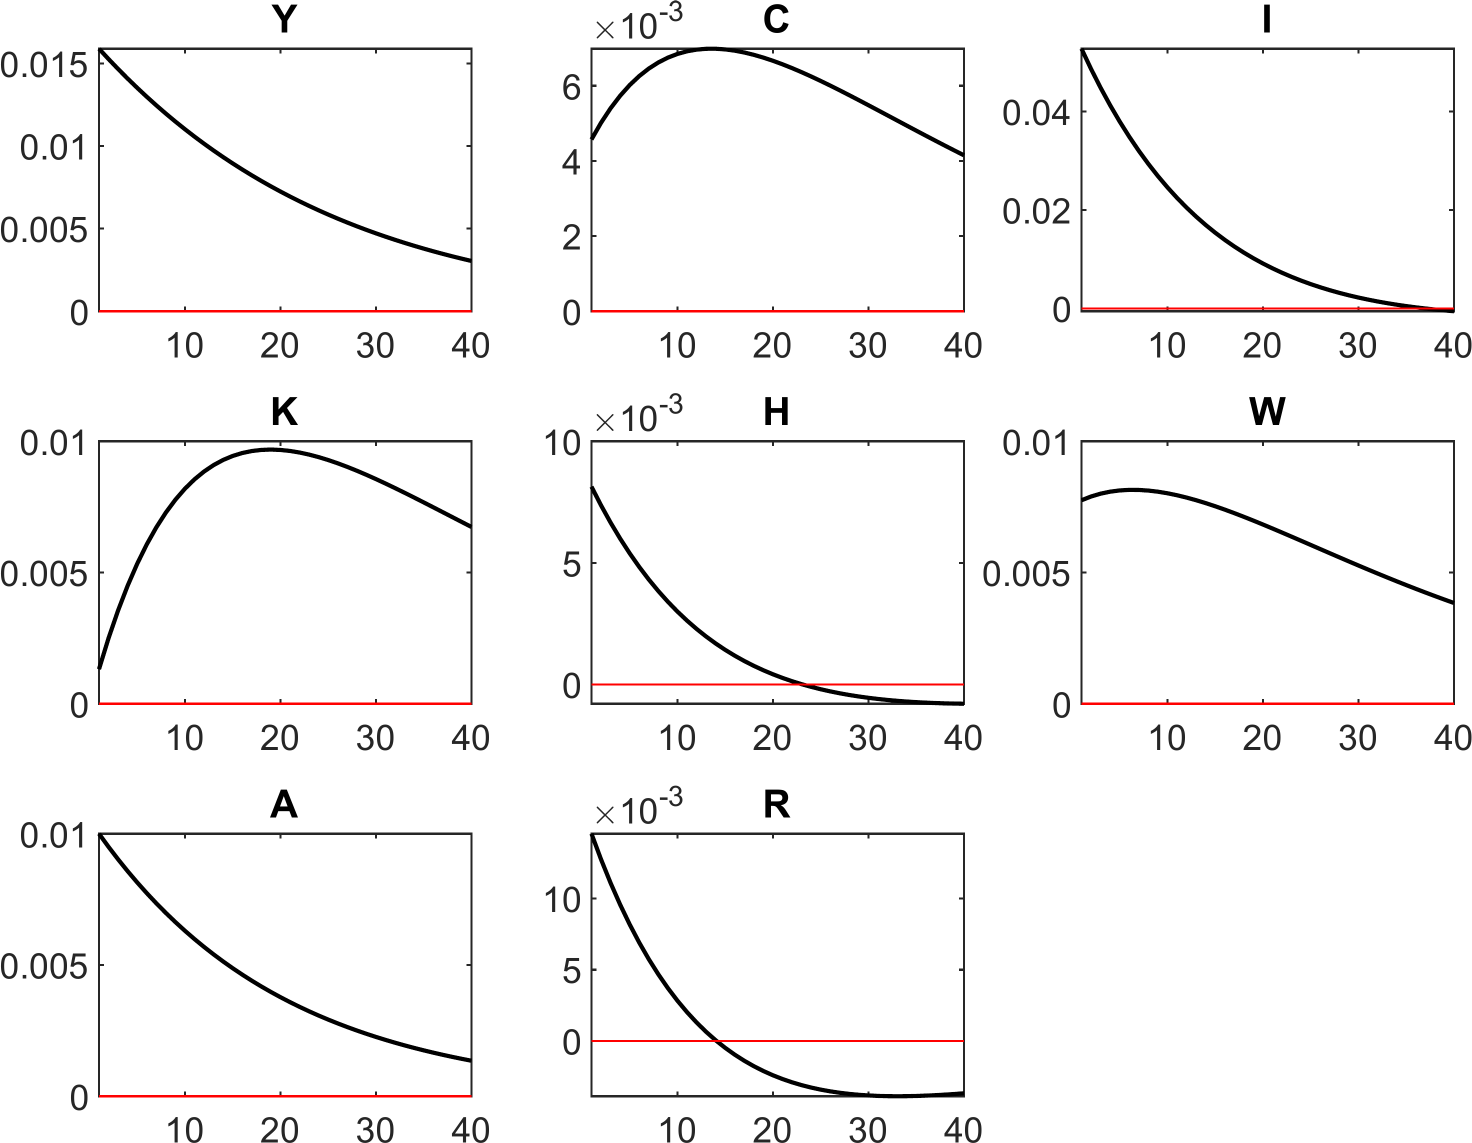
\includegraphics{code/rbc_model/rbc_model/graphs/rbc_model_IRF_eps_cropped.png}
\caption{image}
\end{figure}

\section{Parameterization}\label{parameterization}

\subsection{Calibration Table}\label{calibration-table}

\subsection{Data Alignment}\label{data-alignment}

\section{Quantitative Analysis}\label{quantitative-analysis}

\begin{verbatim}
## [1] "works"
\end{verbatim}

\newpage

\section*{References}\label{references}
\addcontentsline{toc}{section}{References}

\phantomsection\label{refs}
\begin{CSLReferences}{1}{1}
\bibitem[\citeproctext]{ref-Mati2019}
Mati, S. 2019. DynareR: Bringing the power of {Dynare} to {R}, {R
Markdown}, and {Quarto}. \emph{CRAN}. {[}Online{]}, Available:
\url{https://CRAN.R-project.org/package=DynareR}.

\end{CSLReferences}

\bibliography{Tex/ref}





\end{document}
